\subsection{Testing for Credentials Transported over an Encrypted Channel - OTG-AUTHN-001} \label{OTG-AUTHN-001}
\subsubsection{BANK-APP}
\begin{longtable}[l]{ p{2.3cm} | p{.79\linewidth} }\hline
    & \textbf{BANK-APP}
    \hfill CVSS Score: 8.8 \progressbar[filledcolor=red]{0.88}
    \\ \hline
    \textbf{Observation} & After scanning the application with the Vega tool, it was found that the forms in the Registration, Login and Create Transaction pages submit to an insecure HTTP target. Parameters such as User name, Password, TAN number, Account ID are not encrypted. \\
    \textbf{Discovery} &
         Three tools Vega, Burp Suite and cURL were used to discover this vulnerability. Steps are as follows:
            \begin{itemize}
            	\item \textbf{Vega}
            		\begin{itemize}
            			\item Click on the Scan tab and enter the URL to be tested. In our case, it was \code{http://<IP-address>/secure-coding/ \allowbreak public/login.php}.

            			\item Click on the Finish button. A report is generated which has three sections - High, Low, Info. This vulnerability is termed as \code{Clear Password over HTTP} and falls under the High section. See Figure \ref{fig:credentials_over_http}
            		\end{itemize}
            \end{itemize} \\ &
            \begin{itemize}
            	\item After detection, one more tool-the Burp Suite was used to delve deeper into it. \textbf{Burp Suite}
            		\begin{itemize}
            		  \item Open Burp Suite Tool. Click on Proxy tab and set interception to on. This enables us to monitor all requests before being served.

            		  \item Now open the browser and under tools, set Foxy Proxy standard to use Burp Suite for all URLs. On the Login page, enter credentials and click on Submit.

            		  \item Now click on the Proxy tab in the Burp Suite. The requested URL data which contains Username and password can be seen in the Raw tab as plain text; revealing that the request was not encrypted.
            		\end{itemize}
                    
            	\item To verify whether the application works on HTTP or HTTPS, cURL was used. \textbf{cURL}
            		\begin{itemize}
                   		 \item Open the terminal and type \code{curl https://<IP-address>}. The response states unknown protocol.
                		 \item To get a detailed response, use \code{curl --verbose https://<IP-address>}.
                		 \item Now try with \code{curl http://<IP-address>}. The response indicates a successful connection and the output of the request. See Figure \ref{fig:credentials_over_http}. It can be concluded that the application works only on HTTP and does not support transmission over HTTPS.
            		\end{itemize}
            \end{itemize}
    \\
    \textbf{Likelihood} & Likelihood is high since this takes place over the network and is exploitable remotely. Exploitation of this vulnerability requires basic knowledge of any monitoring tools to view the format and details of the server requests. \\
    \textbf{Impact} & A successful attack might lead to serious consequences. The request parameters can be tampered with, as they are not encrypted. This could be used by the attacker to impersonate as the victim, thereby leading to the victim not being able to login or transactions being hijacked. This could result in a Denial of Service attack as well. \\
    \textbf{Recommen\-dations} & It is recommended to use HTTPS for secure communication and also use encryption for the request parameters.\\ \hline
    \textbf{CVSS} &
        \begin{tabular}[t]{@{}l | l}
            Attack Vector           & \textcolor{red}{Network} \\
            Attack Complexity       & \textcolor{red}{Low} \\
            Privileges Required     & \textcolor{BurntOrange}{Low} \\
            User Interaction        & \textcolor{red}{None} \\
            Scope                   & \textcolor{Green}{Unchanged} \\
            Confidentiality Impact  & \textcolor{red}{High} \\
            Integrity Impact        & \textcolor{red}{High} \\
            Availability Impact     & \textcolor{red}{High}
        \end{tabular}
    \\ \hline
\end{longtable}

\subsubsection{SecureBank}
\begin{longtable}[l]{ p{2.3cm} | p{.79\linewidth} }\hline
    & \textbf{SecureBank}
    \hfill CVSS Score: 8.8 \progressbar[filledcolor=red]{0.88}
    \\ \hline
    \textbf{Observation} & After scanning the application with the Vega tool, it was found that the forms in the Registration, Login and Create Transaction pages submit to an insecure HTTP target. Parameters such as User name, Password, TAN number, Account ID are not encrypted. \\
    \textbf{Discovery} & The same vulnerability exists in our application as well; since the channel over which the communication takes place is not encrypted. \\
    \textbf{Likelihood} & Same as described for BANK-APP. \\
    \textbf{Impact} & Same as described for BANK-APP. \\
    \textbf{Recommen\-dations} & Same as described for BANK-APP. \\ \hline
    \textbf{CVSS} & Same as described for BANK-APP.
    \\ \hline
\end{longtable}

\begin{figure}[ht]
	\centering
	\begin{subfigure}{.45\textwidth}
		\centering
		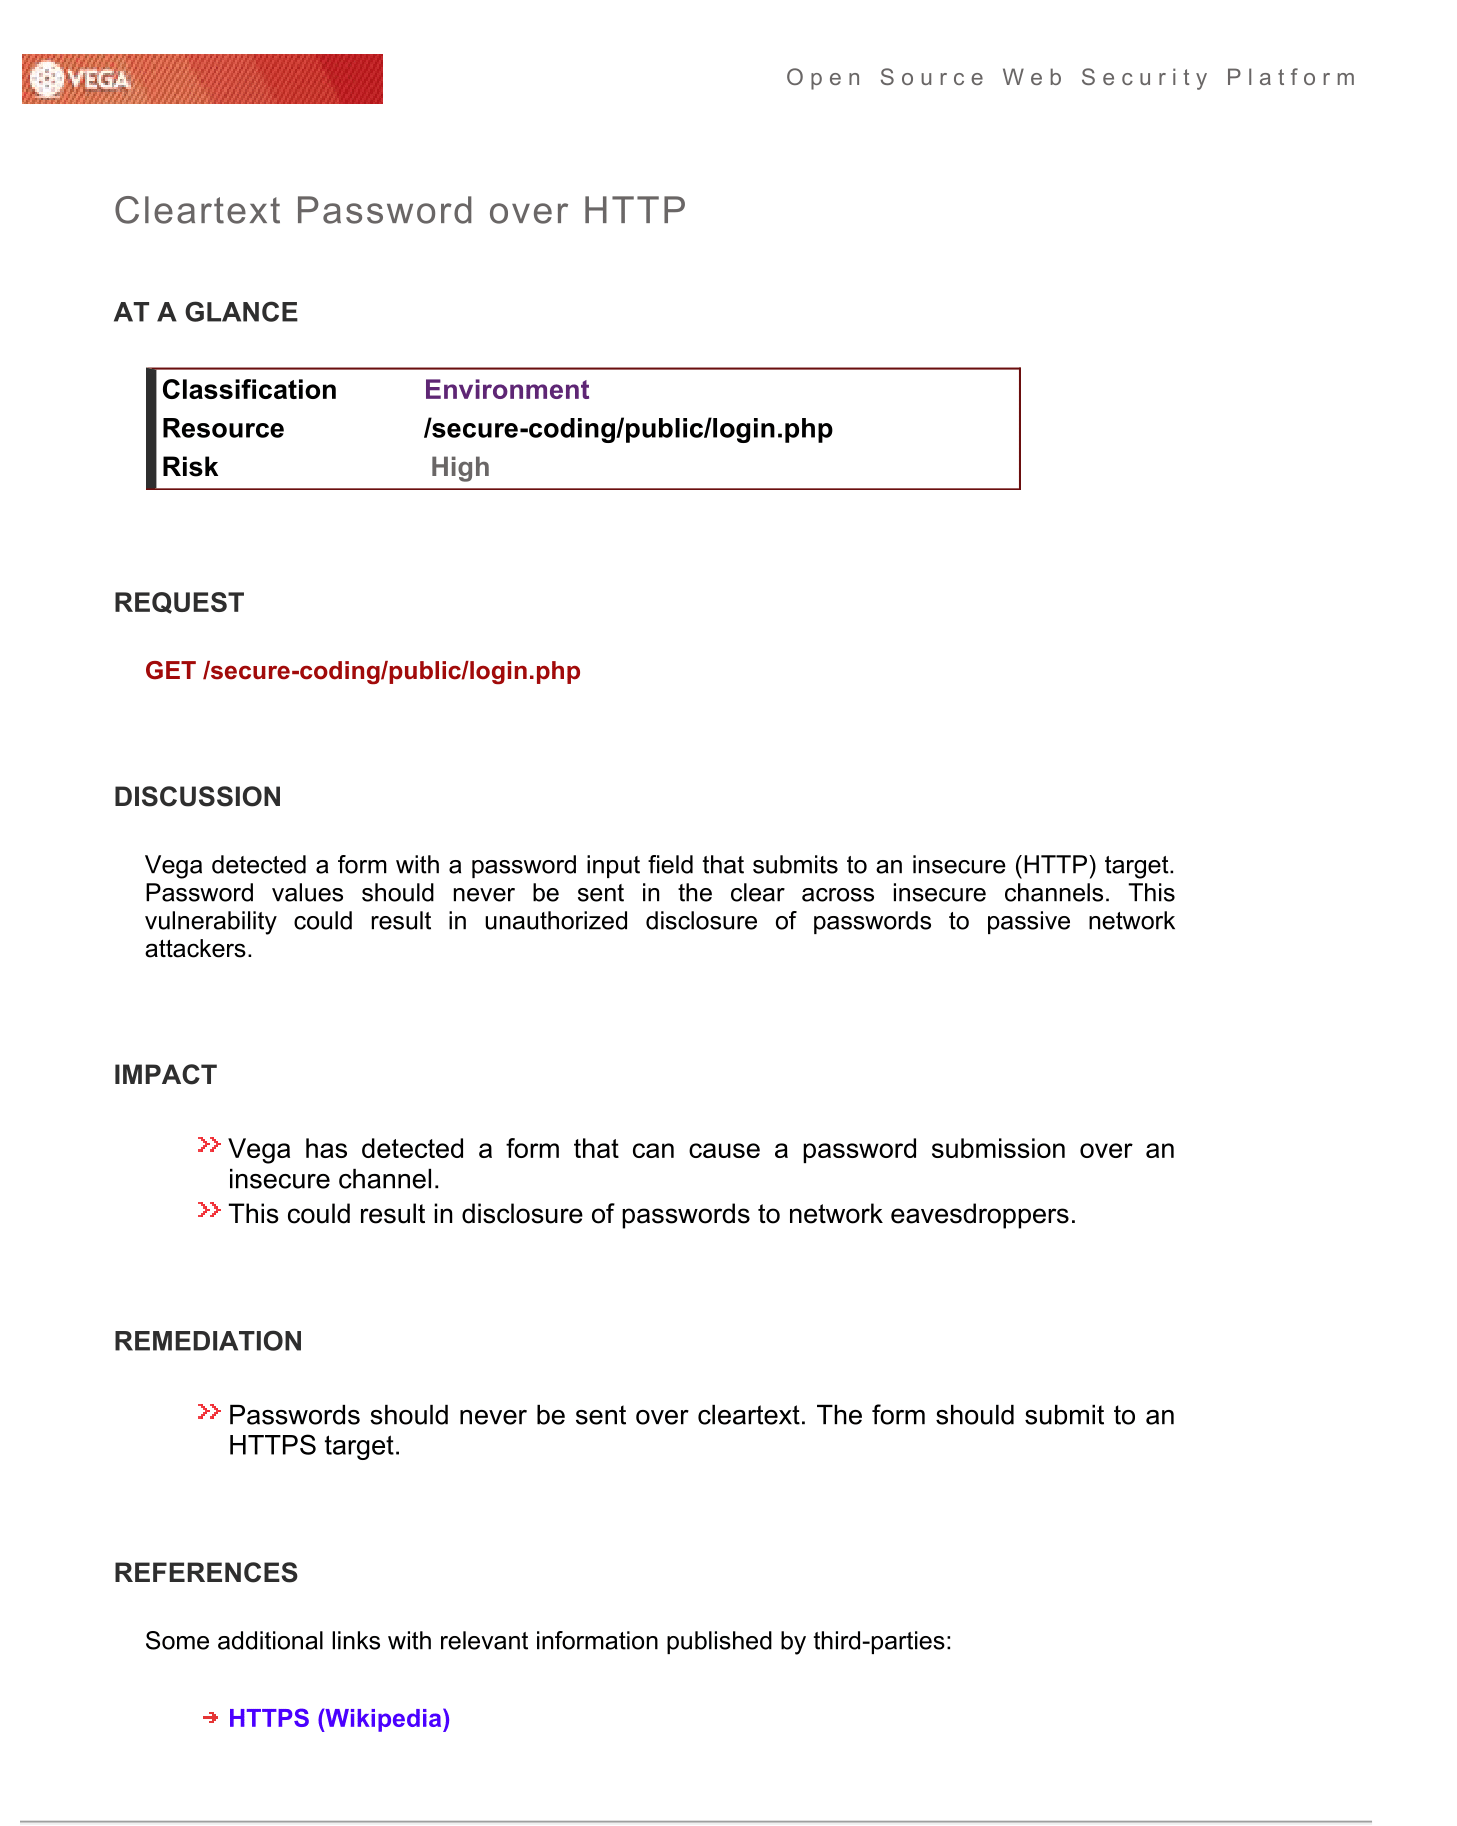
\includegraphics[width=.9\linewidth]{figures/OTG-AUTHN-001_1.png}
		\caption{Vega Report-Clear password over HTTP}
	\end{subfigure}\hfill%
	\begin{subfigure}{.45\textwidth}
		\centering
		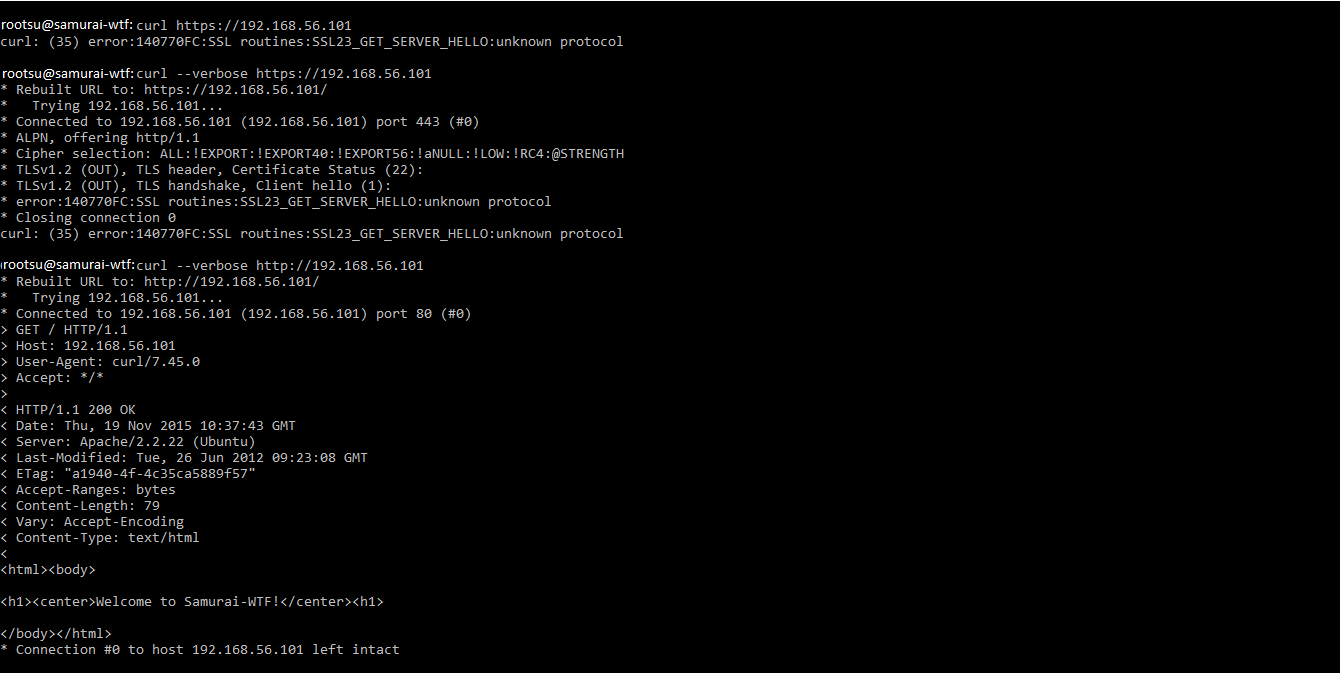
\includegraphics[width=.8\linewidth]{figures/OTG-AUTHN-001_2.png}
		\caption{cURL - Check for HTTPS}
	\end{subfigure}
	\caption{No default credentials for registration}
	\label{fig:credentials_over_http}
\end{figure}

\subsubsection{Comparison}
Both applications behave similarly in transmitting credentials and other confidential data over an insecure HTTP channel.
\clearpage